% abtex2-modelo-trabalho-academico.tex, v-1.9.6 laurocesar
%% Copyright 2012-2016 by abnTeX2 group at http://www.abntex.net.br/ 
%%
%% This work may be distributed and/or modified under the
%% conditions of the LaTeX Project Public License, either version 1.3
%% of this license or (at your option) any later version.
%% The latest version of this license is in
%%   http://www.latex-project.org/lppl.txt
%% and version 1.3 or later is part of all distributions of LaTeX
%% version 2005/12/01 or later.
%%
%% This work has the LPPL maintenance status `maintained'.
%% 
%% The Current Maintainer of this work is the abnTeX2 team, led
%% by Lauro César Araujo. Further information are available on 
%% http://www.abntex.net.br/
%%
%% This work consists of the files abntex2-modelo-trabalho-academico.tex,
%% abntex2-modelo-include-comandos and abntex2-modelo-references.bib
%%

% ------------------------------------------------------------------------
% ------------------------------------------------------------------------
% abnTeX2: Modelo de Trabalho Academico (tese de doutorado, dissertacao de
% mestrado e trabalhos monograficos em geral) em conformidade com 
% ABNT NBR 14724:2011: Informacao e documentacao - Trabalhos academicos -
% Apresentacao
% ------------------------------------------------------------------------
% ------------------------------------------------------------------------

\documentclass[
	% -- opções da classe memoir --
	12pt,				% tamanho da fonte
	%openright,			% capítulos começam em pág ímpar (insere página vazia caso preciso)
	%twoside,			% para impressão em recto e verso. Oposto a oneside
	oneside,			% impressão de um lado só
	a4paper,			% tamanho do papel. 
	% -- opções da classe abntex2 --
	chapter=TITLE,		% títulos de capítulos convertidos em letras maiúsculas
	section=TITLE,		% títulos de seções convertidos em letras maiúsculas
	%subsection=TITLE,	% títulos de subseções convertidos em letras maiúsculas
	%subsubsection=TITLE,% títulos de subsubseções convertidos em letras maiúsculas
	sumario=abnt-6027-2012, % opção de sumário
	%sumario=tradicional,
	% -- opções do pacote babel --
	english,			% idioma adicional para hifenização
	french,				% idioma adicional para hifenização
	spanish,			% idioma adicional para hifenização
	brazil				% o último idioma é o principal do documento
	]{abntex2}

% ---
% Pacotes básicos 
% ---
\usepackage{lmodern}			% Usa a fonte Latin Modern			
\usepackage[T1]{fontenc}		% Selecao de codigos de fonte.
\usepackage[utf8]{inputenc}		% Codificacao do documento (conversão automática dos acentos)
\usepackage{lastpage}			% Usado pela Ficha catalográfica
\usepackage{indentfirst}		% Indenta o primeiro parágrafo de cada seção.
\usepackage{color}				% Controle das cores
\usepackage{graphicx}			% Inclusão de gráficos
\usepackage{microtype} 			% Melhorias de justificação
\usepackage{hyperref}
\usepackage{facens}				% Padrão Facens
\usepackage{pdfpages}			% Include de pdfs
\usepackage{lipsum}				% Geração de dummy text
\usepackage[alf]{abntex2cite}	% Citações padrão ABNT
%\usepackage[brazilian,hyperpageref]{backref}	 % Paginas com as citações na bibl
\usepackage{listings}

% Estilo do Listing
% frame = (none|leftline|topline|bottomline|lines|single|shadowbox)
\lstset{
basicstyle=\fontfamily{pcr}\selectfont\footnotesize,
breaklines=true, 
frame=single}
% ---

% ---
% Indicando pasta de figuras\\
% ---
\graphicspath{{imagens/}}
% ---

% --- 
% CONFIGURAÇÕES DE PACOTES
% --- 

% ---
% Configurações do pacote backref
% Usado sem a opção hyperpageref de backref
%\renewcommand{\backrefpagesname}{Citado na(s) página(s):~}
% Texto padrão antes do número das páginas
%\renewcommand{\backref}{}
% Define os textos da citação
%\renewcommand*{\backrefalt}[4]{
%	\ifcase #1 %
%		Nenhuma citação no texto.%
%	\or
%		Citado na página #2.%
%	\else
%		Citado #1 vezes nas páginas #2.%
%	\fi}%
% ---

% ---
% Informações de dados para CAPA e FOLHA DE ROSTO
% ---
\titulo{Plataforma gamificada de treinamento empresarial}
\autor{Gustavo Sanches \\ Rafael Zabeu Spessotto}
\local{Sorocaba/SP}
\data{2019}
\orientador{Johannes von Lochter}
\instituicao{Faculdade de Engenharia de Sorocaba - FACENS}
\tipotrabalho{Dissertação}

% O preambulo deve conter o tipo do trabalho, o objetivo, 
% o nome da instituição e a área de concentração 
\preambulo{}
% ---

\counterwithin{figure}{chapter}
\counterwithin{table}{chapter}
\counterwithin{quadro}{chapter}

% ---
% Configurações de aparência do PDF final

% alterando o aspecto da cor azul
\definecolor{blue}{RGB}{41,5,195}

% informações do PDF
\makeatletter
\hypersetup{
     	%pagebackref=true,
		pdftitle={\@title}, 
		pdfauthor={\@author},
    	pdfsubject={\imprimirpreambulo},
	    pdfcreator={LaTeX with abnTeX2},
		pdfkeywords={abnt}{latex}{abntex}{abntex2}{trabalho acadêmico}, 
		colorlinks=false,       		% false: boxed links; true: colored links
    	linkcolor=blue,          	% color of internal links
    	citecolor=blue,        		% color of links to bibliography
    	filecolor=magenta,      		% color of file links
		urlcolor=blue,
		bookmarksdepth=4
}
\makeatother
% --- 

% --- 
% Espaçamentos entre linhas e parágrafos 
% --- 

% O tamanho do parágrafo é dado por:
\setlength{\parindent}{1.25cm}

% Controle do espaçamento entre um parágrafo e outro:
\setlength{\parskip}{0.2cm}  % tente também \onelineskip

% ---
% compila o indice
% ---
\makeindex
% ---

% ----
% Início do documento
% ----
\begin{document}

% Seleciona o idioma do documento (conforme pacotes do babel)
%\selectlanguage{english}
\selectlanguage{brazil}

% Retira espaço extra obsoleto entre as frases.
\frenchspacing 

% ----------------------------------------------------------
% ELEMENTOS PRÉ-TEXTUAIS
% ----------------------------------------------------------
\pretextual

%\includepdf{report6.pdf}


% ---
% Capa
% ---
\imprimircapa
% ---

% ---
% Folha de rosto
% (o * indica que haverá a ficha bibliográfica)
% ---
\imprimirfolhaderosto*
% ---

% ---
% Inserir a ficha bibliografica
% ---

% Isto é um exemplo de Ficha Catalográfica, ou ``Dados internacionais de
% catalogação-na-publicação''. Você pode utilizar este modelo como referência. 
% Porém, provavelmente a biblioteca da sua universidade lhe fornecerá um PDF
% com a ficha catalográfica definitiva após a defesa do trabalho. Quando estiver
% com o documento, salve-o como PDF no diretório do seu projeto e substitua todo
% o conteúdo de implementação deste arquivo pelo comando abaixo:
%
% \begin{fichacatalografica}
%     \includepdf{fichacatalografica.pdf}
% \end{fichacatalografica}

%\begin{fichacatalografica}
	\sffamily
	\vspace*{\fill}					% Posição vertical
	\begin{center}					% Minipage Centralizado
	\fbox{\begin{minipage}[c][8cm]{13.5cm}		% Largura
	\small
	\imprimirautor
	%Sobrenome, Nome do autor
	
	\hspace{0.5cm} \imprimirtitulo  / \imprimirautor. --
	\imprimirlocal, \imprimirdata-
	
	\hspace{0.5cm} \pageref{LastPage} p. : il. (algumas color.) ; 30 cm.\\
	
	\hspace{0.5cm} \imprimirorientadorRotulo~\imprimirorientador\\
	
	\hspace{0.5cm}
	\parbox[t]{\textwidth}{\imprimirtipotrabalho~--~\imprimirinstituicao,
	\imprimirdata.}\\
	
	\hspace{0.5cm}
		1. IoT.
		2. CQRS.
		2. Big Data.
		I. Trânsito.
		II. Me. Andréia Damasio de Leles.
		III. Faculdade de Engenharia de Sorocaba.
		IV. Um Sistema de Iot Para Urgências no Trânsito 			
	\end{minipage}}
	\end{center}
\end{fichacatalografica}
% ---

% ---
% Inserir errata
% ---
%\begin{errata}
Elemento opcional da \citeonline[4.2.1.2]{NBR14724:2011}. Exemplo:

\vspace{\onelineskip}

FERRIGNO, C. R. A. \textbf{Tratamento de neoplasias ósseas apendiculares com
reimplantação de enxerto ósseo autólogo autoclavado associado ao plasma
rico em plaquetas}: estudo crítico na cirurgia de preservação de membro em
cães. 2011. 128 f. Tese (Livre-Docência) - Faculdade de Medicina Veterinária e
Zootecnia, Universidade de São Paulo, São Paulo, 2011.

\begin{table}[htb]
\center
\footnotesize
\begin{tabular}{|p{1.4cm}|p{1cm}|p{3cm}|p{3cm}|}
  \hline
   \textbf{Folha} & \textbf{Linha}  & \textbf{Onde se lê}  & \textbf{Leia-se}  \\
    \hline
    1 & 10 & auto-conclavo & autoconclavo\\
   \hline
\end{tabular}
\end{table}

\end{errata}
% ---

% ---
% Inserir folha de aprovação
% ---

% Isto é um exemplo de Folha de aprovação, elemento obrigatório da NBR
% 14724/2011 (seção 4.2.1.3). Você pode utilizar este modelo até a aprovação
% do trabalho. Após isso, substitua todo o conteúdo deste arquivo por uma
% imagem da página assinada pela banca com o comando abaixo:
%
% \includepdf{folhadeaprovacao_final.pdf}
%
%\begin{folhadeaprovacao}

  \begin{center}
    {\ABNTEXchapterfont\large\textbf{\imprimirautor}}

    \vspace*{\fill}\vspace*{\fill}
    \begin{center}
      \ABNTEXchapterfont\bfseries\Large\imprimirtitulo
    \end{center}
    \vspace*{\fill}
    
    \hspace{.45\textwidth}
    \begin{minipage}{.5\textwidth}
        \imprimirpreambulo
    \end{minipage}%
    \vspace*{\fill}
   \end{center}
        
   \imprimirlocal, 12 de Dezembro de 2017.

   \assinatura{Orientadora \textbf{\imprimirorientador}} 
   \assinatura{\textbf{Professor} Convidado 1}
   \assinatura{\textbf{Professor} Convidado 2}
   %\assinatura{\textbf{Professor} \\ Convidado 3}
   %\assinatura{\textbf{Professor} \\ Convidado 4}
      
%   \begin{center}
%    \vspace*{0.5cm}
%    {\large\imprimirlocal}
%    \par
%    {\large\imprimirdata}
%    \vspace*{1cm}
%  \end{center}
  
\end{folhadeaprovacao}
% ---

% ---
% Dedicatória
% ---
%\begin{dedicatoria}
   \vspace*{\fill}
   \centering
   \noindent
   \textit{ Este trabalho é dedicado às crianças adultas que,\\
   quando pequenas, sonharam em se tornar cientistas.} \vspace*{\fill}
\end{dedicatoria}
% ---

% ---
% Agradecimentos
% ---
\begin{agradecimentos}

\end{agradecimentos}
%\begin{agradecimentos}

\end{agradecimentos}
% ---

% ---
% Epígrafe
% ---
\begin{epigrafe}
    \vspace*{\fill}
	\begin{flushright}
		\textit{<Epígrafe>}
	\end{flushright}
\end{epigrafe}
% ---

% ---
% RESUMOS
% ---

% resumo em português
\setlength{\absparsep}{18pt} % ajusta o espaçamento dos parágrafos do resumo
\begin{resumo}
O objetivo do projeto é desenvolver uma aplicação de aprendizado gamificada para
empresas utilizarem como reforço e incentivo para aprendizado de tópicos.

A aplicação permitiria a empresa criar questões sobre um assunto que considere
interessante e acompanhar quantas pessoas acertaram e erraram cada questão, podendo
assim verificar quanto esse assunto é dominado pelos participantes e acompanhar o
progresso do aprendizado em geral.

Sendo uma plataforma gamificada os usuários são incentivados a jogar para subir
no ranking geral, e respondendo as perguntas vai gradualmente aprendendo e reforçando
os conhecimentos desejados.

A aplicação teria um servidor para guardar as informações e coordenar os jogos,
clientes em PC, Android e IOS onde o jogo será jogado e uma aplicação web como
dashboard administrativo.


 \textbf{Palavras-chave}: Gamificação. Indústria. Unity3D. Lúdico.
\end{resumo}

% resumo em inglês
\setlength{\absparsep}{18pt} % ajusta o espaçamento dos parágrafos do resumo
\begin{resumo}[Abstract]


 \textbf{Keywords}: Gamificação, Indústria, Unity3D, Lúdico.
\end{resumo}

% ---

% ---
% inserir lista de ilustrações
% ---
\pdfbookmark[0]{\listfigurename}{lof}
%\listoffigures*
\cleardoublepage
% ---

% ---
% Lista de Quadros
% ---
%\pdfbookmark[0]{\listofquadrosname}{loq}
\listofquadros*
\cleardoublepage
% ---

% ---
% inserir lista de tabelas
% ---
%\pdfbookmark[0]{\listtablename}{lot}
\listoftables*
\cleardoublepage
% ---

% ---
% inserir lista de abreviaturas e siglas
% ---
\begin{siglas}
  \item[IoT] \textit{Internet of Things}
%  \item[RFID] \textit{Radio-Frequency IDentification}
%  \item[V2V] \textit{Vehicle to Vehicle}
%  \item[V2I] \textit{Vehicle to Infrastructure}
%  \item[DOT] Departamento de Transportes do Estados Unidos
%  \item[IP]  \textit{Internal Protocol}
%  \item[TIC] Tecnologia da Informação e Comunicação
%  \item[IDC] \textit{Digital Universe Study}
%  \item[HDFS] \textit{Hadoop Distributed File System}
%  \item[API] \textit{Application Programming Interface}
%  \item[JVM] \textit{Java Virtual Machine}
%  \item[Saas] \textit{Software as a Service}
%  \item[CQRS] \textit{Command Query Responsibility Segregation}
%  \item[JSON] \textit{JavaScript Object Notation}
%  \item[JRE] \textit{Java SE Runtime Environment}
%  \item[SaaS] \textit{Server as a Service}
\end{siglas}
% ---

% ---
% inserir lista de símbolos
% ---
%\begin{simbolos}
  \item[$ \Gamma $] Letra grega Gama
  \item[$ \Lambda $] Lambda
  \item[$ \zeta $] Letra grega minúscula zeta
  \item[$ \in $] Pertence
\end{simbolos}
% ---

% ---
% inserir o sumario
% ---
\pdfbookmark[0]{\contentsname}{toc}
\tableofcontents*
\cleardoublepage
% ---



% ----------------------------------------------------------
% ELEMENTOS TEXTUAIS
% ----------------------------------------------------------
\textual
\pagestyle{simple}
% ----------------------------------------------------------
% Introdução (exemplo de capítulo sem numeração, mas presente no Sumário)
% ----------------------------------------------------------
\chapter{Introdução}
%\addcontentsline{toc}{chapter}{Introdução}


% ----------------------------------------------------------
% PARTE
% ----------------------------------------------------------
%\part{Preparação da pesquisa}

% ----------------------------------------------------------

% ---
% Capitulo com exemplos de comandos inseridos de arquivo externo 
% ---
%%% abtex2-modelo-include-comandos.tex, v-1.9.6 laurocesar
%% Copyright 2012-2016 by abnTeX2 group at http://www.abntex.net.br/ 
%%
%% This work may be distributed and/or modified under the
%% conditions of the LaTeX Project Public License, either version 1.3
%% of this license or (at your option) any later version.
%% The latest version of this license is in
%%   http://www.latex-project.org/lppl.txt
%% and version 1.3 or later is part of all distributions of LaTeX
%% version 2005/12/01 or later.
%%
%% This work has the LPPL maintenance status `maintained'.
%% 
%% The Current Maintainer of this work is the abnTeX2 team, led
%% by Lauro César Araujo. Further information are available on 
%% http://www.abntex.net.br/
%%
%% This work consists of the files abntex2-modelo-include-comandos.tex
%% and abntex2-modelo-img-marca.pdf
%%

% ---
% Este capítulo, utilizado por diferentes exemplos do abnTeX2, ilustra o uso de
% comandos do abnTeX2 e de LaTeX.
% ---
 
\chapter{Resultados de comandos}\label{cap_exemplos}

\chapterprecis{Isto é uma sinopse de capítulo. A ABNT não traz nenhuma
normatização a respeito desse tipo de resumo, que é mais comum em romances 
e livros técnicos.}\index{sinopse de capítulo}

% ---
\section{Codificação dos arquivos: UTF8}
% ---

A codificação de todos os arquivos do \abnTeX\ é \texttt{UTF8}. É necessário que
você utilize a mesma codificação nos documentos que escrever, inclusive nos
arquivos de base bibliográficas |.bib|.

% ---
\section{Citações diretas}
\label{sec-citacao}
% ---

\index{citações!diretas}Utilize o ambiente \texttt{citacao} para incluir
citações diretas com mais de três linhas:

\begin{citacao}
As citações diretas, no texto, com mais de três linhas, devem ser
destacadas com recuo de 4 cm da margem esquerda, com letra menor que a do texto
utilizado e sem as aspas. No caso de documentos datilografados, deve-se
observar apenas o recuo \cite[5.3]{NBR10520:2002}.
\end{citacao}

Use o ambiente assim:

\begin{verbatim}
\begin{citacao}
As citações diretas, no texto, com mais de três linhas [...] deve-se observar
apenas o recuo \cite[5.3]{NBR10520:2002}.
\end{citacao}
\end{verbatim}

O ambiente \texttt{citacao} pode receber como parâmetro opcional um nome de
idioma previamente carregado nas opções da classe (\autoref{sec-hifenizacao}). Nesse
caso, o texto da citação é automaticamente escrito em itálico e a hifenização é
ajustada para o idioma selecionado na opção do ambiente. Por exemplo:

\begin{verbatim}
\begin{citacao}[english]
Text in English language in italic with correct hyphenation.
\end{citacao}
\end{verbatim}

Tem como resultado:

\begin{citacao}[english]
Text in English language in italic with correct hyphenation.
\end{citacao}

\index{citações!simples}Citações simples, com até três linhas, devem ser
incluídas com aspas. Observe que em \LaTeX as aspas iniciais são diferentes das
finais: ``Amor é fogo que arde sem se ver''.

% ---
\section{Notas de rodapé}
% ---

As notas de rodapé são detalhadas pela NBR 14724:2011 na seção 5.2.1\footnote{As
notas devem ser digitadas ou datilografadas dentro das margens, ficando
separadas do texto por um espaço simples de entre as linhas e por filete de 5
cm, a partir da margem esquerda. Devem ser alinhadas, a partir da segunda linha
da mesma nota, abaixo da primeira letra da primeira palavra, de forma a destacar
o expoente, sem espaço entre elas e com fonte menor
\citeonline[5.2.1]{NBR14724:2011}.}\footnote{Caso uma série de notas sejam
criadas sequencialmente, o \abnTeX\ instrui o \LaTeX\ para que uma vírgula seja
colocada após cada número do expoente que indica a nota de rodapé no corpo do
texto.}\footnote{Verifique se os números do expoente possuem uma vírgula para
dividi-los no corpo do texto.}. 


% ---
\section{Tabelas}
% ---

\index{tabelas}A \autoref{tab-nivinv} é um exemplo de tabela construída em
\LaTeX.

\begin{table}[htb]
\ABNTEXfontereduzida
\caption[Níveis de investigação]{Níveis de investigação.}
\label{tab-nivinv}
\begin{tabular}{p{2.6cm}|p{6.0cm}|p{2.25cm}|p{3.40cm}}
  %\hline
   \textbf{Nível de Investigação} & \textbf{Insumos}  & \textbf{Sistemas de Investigação}  & \textbf{Produtos}  \\
    \hline
    Meta-nível & Filosofia\index{filosofia} da Ciência  & Epistemologia &
    Paradigma  \\
    \hline
    Nível do objeto & Paradigmas do metanível e evidências do nível inferior &
    Ciência  & Teorias e modelos \\
    \hline
    Nível inferior & Modelos e métodos do nível do objeto e problemas do nível inferior & Prática & Solução de problemas  \\
   % \hline
\end{tabular}
\legend{Fonte: \citeonline{van86}}
\end{table}

Já a \autoref{tabela-ibge} apresenta uma tabela criada conforme o padrão do
\citeonline{ibge1993} requerido pelas normas da ABNT para documentos técnicos e
acadêmicos.

\begin{table}[htb]
\IBGEtab{%
  \caption{Um Exemplo de tabela alinhada que pode ser longa
  ou curta, conforme padrão IBGE.}%
  \label{tabela-ibge}
}{%
  \begin{tabular}{ccc}
  \toprule
   Nome & Nascimento & Documento \\
  \midrule \midrule
   Maria da Silva & 11/11/1111 & 111.111.111-11 \\
  \midrule 
   João Souza & 11/11/2111 & 211.111.111-11 \\
  \midrule 
   Laura Vicuña & 05/04/1891 & 3111.111.111-11 \\
  \bottomrule
\end{tabular}%
}{%
  \fonte{Produzido pelos autores.}%
  \nota{Esta é uma nota, que diz que os dados são baseados na
  regressão linear.}%
  \nota[Anotações]{Uma anotação adicional, que pode ser seguida de várias
  outras.}%
  }
\end{table}


% ---
\section{Figuras}
% ---

\index{figuras}Figuras podem ser criadas diretamente em \LaTeX,
como o exemplo da \autoref{fig_circulo}.

\begin{figure}[htb]
	\caption{\label{fig_circulo}A delimitação do espaço}
	\begin{center}
	    \setlength{\unitlength}{5cm}
		\begin{picture}(1,1)
		\put(0,0){\line(0,1){1}}
		\put(0,0){\line(1,0){1}}
		\put(0,0){\line(1,1){1}}
		\put(0,0){\line(1,2){.5}}
		\put(0,0){\line(1,3){.3333}}
		\put(0,0){\line(1,4){.25}}
		\put(0,0){\line(1,5){.2}}
		\put(0,0){\line(1,6){.1667}}
		\put(0,0){\line(2,1){1}}
		\put(0,0){\line(2,3){.6667}}
		\put(0,0){\line(2,5){.4}}
		\put(0,0){\line(3,1){1}}
		\put(0,0){\line(3,2){1}}
		\put(0,0){\line(3,4){.75}}
		\put(0,0){\line(3,5){.6}}
		\put(0,0){\line(4,1){1}}
		\put(0,0){\line(4,3){1}}
		\put(0,0){\line(4,5){.8}}
		\put(0,0){\line(5,1){1}}
		\put(0,0){\line(5,2){1}}
		\put(0,0){\line(5,3){1}}
		\put(0,0){\line(5,4){1}}
		\put(0,0){\line(5,6){.8333}}
		\put(0,0){\line(6,1){1}}
		\put(0,0){\line(6,5){1}}
		\end{picture}
	\end{center}
	\legend{Fonte: os autores}
\end{figure}

Ou então figuras podem ser incorporadas de arquivos externos, como é o caso da
\autoref{fig_grafico}. Se a figura que ser incluída se tratar de um diagrama, um
gráfico ou uma ilustração que você mesmo produza, priorize o uso de imagens
vetoriais no formato PDF. Com isso, o tamanho do arquivo final do trabalho será
menor, e as imagens terão uma apresentação melhor, principalmente quando
impressas, uma vez que imagens vetorias são perfeitamente escaláveis para
qualquer dimensão. Nesse caso, se for utilizar o Microsoft Excel para produzir
gráficos, ou o Microsoft Word para produzir ilustrações, exporte-os como PDF e
os incorpore ao documento conforme o exemplo abaixo. No entanto, para manter a
coerência no uso de software livre (já que você está usando \LaTeX e \abnTeX),
teste a ferramenta \textsf{InkScape}\index{InkScape}
(\url{http://inkscape.org/}). Ela é uma excelente opção de código-livre para
produzir ilustrações vetoriais, similar ao CorelDraw\index{CorelDraw} ou ao Adobe
Illustrator\index{Adobe Illustrator}. De todo modo, caso não seja possível
utilizar arquivos de imagens como PDF, utilize qualquer outro formato, como
JPEG, GIF, BMP, etc. Nesse caso, você pode tentar aprimorar as imagens
incorporadas com o software livre \textsf{Gimp}\index{Gimp}
(\url{http://www.gimp.org/}). Ele é uma alternativa livre ao Adobe
Photoshop\index{Adobe Photoshop}.

\begin{figure}[htb]
	\caption{\label{fig_grafico}Gráfico produzido em Excel e salvo como PDF}
	\begin{center}
	    \includegraphics[scale=0.5]{abntex2-modelo-img-grafico.pdf}
	\end{center}
	\legend{Fonte: \citeonline[p. 24]{araujo2012}}
\end{figure}

% ---
\subsection{Figuras em \emph{minipages}}
% ---

\emph{Minipages} são usadas para inserir textos ou outros elementos em quadros
com tamanhos e posições controladas. Veja o exemplo da
\autoref{fig_minipage_imagem1} e da \autoref{fig_minipage_grafico2}.

\begin{figure}[htb]
 \label{teste}
 \centering
  \begin{minipage}{0.4\textwidth}
    \centering
    \caption{Imagem 1 da minipage} \label{fig_minipage_imagem1}
    \includegraphics[scale=0.9]{abntex2-modelo-img-marca.pdf}
    \legend{Fonte: Produzido pelos autores}
  \end{minipage}
  \hfill
  \begin{minipage}{0.4\textwidth}
    \centering
    \caption{Grafico 2 da minipage} \label{fig_minipage_grafico2}
    \includegraphics[scale=0.2]{abntex2-modelo-img-grafico.pdf}
    \legend{Fonte: \citeonline[p. 24]{araujo2012}}
  \end{minipage}
\end{figure}

Observe que, segundo a \citeonline[seções 4.2.1.10 e 5.8]{NBR14724:2011}, as
ilustrações devem sempre ter numeração contínua e única em todo o documento:

\begin{citacao}
Qualquer que seja o tipo de ilustração, sua identificação aparece na parte
superior, precedida da palavra designativa (desenho, esquema, fluxograma,
fotografia, gráfico, mapa, organograma, planta, quadro, retrato, figura,
imagem, entre outros), seguida de seu número de ordem de ocorrência no texto,
em algarismos arábicos, travessão e do respectivo título. Após a ilustração, na
parte inferior, indicar a fonte consultada (elemento obrigatório, mesmo que
seja produção do próprio autor), legenda, notas e outras informações
necessárias à sua compreensão (se houver). A ilustração deve ser citada no
texto e inserida o mais próximo possível do trecho a que se
refere. \cite[seções 5.8]{NBR14724:2011}
\end{citacao}

% ---
\section{Expressões matemáticas}
% ---

\index{expressões matemáticas}Use o ambiente \texttt{equation} para escrever
expressões matemáticas numeradas:

\begin{equation}
  \forall x \in X, \quad \exists \: y \leq \epsilon
\end{equation}

Escreva expressões matemáticas entre \$ e \$, como em $ \lim_{x \to \infty}
\exp(-x) = 0 $, para que fiquem na mesma linha.

Também é possível usar colchetes para indicar o início de uma expressão
matemática que não é numerada.

\[
\left|\sum_{i=1}^n a_ib_i\right|
\le
\left(\sum_{i=1}^n a_i^2\right)^{1/2}
\left(\sum_{i=1}^n b_i^2\right)^{1/2}
\]

Consulte mais informações sobre expressões matemáticas em
\url{https://github.com/abntex/abntex2/wiki/Referencias}.

% ---
\section{Enumerações: alíneas e subalíneas}
% ---

\index{alíneas}\index{subalíneas}\index{incisos}Quando for necessário enumerar
os diversos assuntos de uma seção que não possua título, esta deve ser
subdividida em alíneas \cite[4.2]{NBR6024:2012}:

\begin{alineas}

  \item os diversos assuntos que não possuam título próprio, dentro de uma mesma
  seção, devem ser subdivididos em alíneas; 
  
  \item o texto que antecede as alíneas termina em dois pontos;
  \item as alíneas devem ser indicadas alfabeticamente, em letra minúscula,
  seguida de parêntese. Utilizam-se letras dobradas, quando esgotadas as
  letras do alfabeto;

  \item as letras indicativas das alíneas devem apresentar recuo em relação à
  margem esquerda;

  \item o texto da alínea deve começar por letra minúscula e terminar em
  ponto-e-vírgula, exceto a última alínea que termina em ponto final;

  \item o texto da alínea deve terminar em dois pontos, se houver subalínea;

  \item a segunda e as seguintes linhas do texto da alínea começa sob a
  primeira letra do texto da própria alínea;
  
  \item subalíneas \cite[4.3]{NBR6024:2012} devem ser conforme as alíneas a
  seguir:

  \begin{alineas}
     \item as subalíneas devem começar por travessão seguido de espaço;

     \item as subalíneas devem apresentar recuo em relação à alínea;

     \item o texto da subalínea deve começar por letra minúscula e terminar em
     ponto-e-vírgula. A última subalínea deve terminar em ponto final, se não
     houver alínea subsequente;

     \item a segunda e as seguintes linhas do texto da subalínea começam sob a
     primeira letra do texto da própria subalínea.
  \end{alineas}
  
  \item no \abnTeX\ estão disponíveis os ambientes \texttt{incisos} e
  \texttt{subalineas}, que em suma são o mesmo que se criar outro nível de
  \texttt{alineas}, como nos exemplos à seguir:
  
  \begin{incisos}
    \item \textit{Um novo inciso em itálico};
  \end{incisos}
  
  \item Alínea em \textbf{negrito}:
  
  \begin{subalineas}
    \item \textit{Uma subalínea em itálico};
    \item \underline{\textit{Uma subalínea em itálico e sublinhado}}; 
  \end{subalineas}
  
  \item Última alínea com \emph{ênfase}.
  
\end{alineas}

% ---
\section{Espaçamento entre parágrafos e linhas}
% ---

\index{espaçamento!dos parágrafos}O tamanho do parágrafo, espaço entre a margem
e o início da frase do parágrafo, é definido por:

\begin{verbatim}
   \setlength{\parindent}{1.3cm}
\end{verbatim}

\index{espaçamento!do primeiro parágrafo}Por padrão, não há espaçamento no
primeiro parágrafo de cada início de divisão do documento
(\autoref{sec-divisoes}). Porém, você pode definir que o primeiro parágrafo
também seja indentado, como é o caso deste documento. Para isso, apenas inclua o
pacote \textsf{indentfirst} no preâmbulo do documento:

\begin{verbatim}
   \usepackage{indentfirst}      % Indenta o primeiro parágrafo de cada seção.
\end{verbatim}

\index{espaçamento!entre os parágrafos}O espaçamento entre um parágrafo e outro
pode ser controlado por meio do comando:

\begin{verbatim}
  \setlength{\parskip}{0.2cm}  % tente também \onelineskip
\end{verbatim}

\index{espaçamento!entre as linhas}O controle do espaçamento entre linhas é
definido por:

\begin{verbatim}
  \OnehalfSpacing       % espaçamento um e meio (padrão); 
  \DoubleSpacing        % espaçamento duplo
  \SingleSpacing        % espaçamento simples	
\end{verbatim}

Para isso, também estão disponíveis os ambientes:

\begin{verbatim}
  \begin{SingleSpace} ...\end{SingleSpace}
  \begin{Spacing}{hfactori} ... \end{Spacing}
  \begin{OnehalfSpace} ... \end{OnehalfSpace}
  \begin{OnehalfSpace*} ... \end{OnehalfSpace*}
  \begin{DoubleSpace} ... \end{DoubleSpace}
  \begin{DoubleSpace*} ... \end{DoubleSpace*} 
\end{verbatim}

Para mais informações, consulte \citeonline[p. 47-52 e 135]{memoir}.

% ---
\section{Inclusão de outros arquivos}\label{sec-include}
% ---

É uma boa prática dividir o seu documento em diversos arquivos, e não
apenas escrever tudo em um único. Esse recurso foi utilizado neste
documento. Para incluir diferentes arquivos em um arquivo principal,
de modo que cada arquivo incluído fique em uma página diferente, utilize o
comando:

\begin{verbatim}
   \include{documento-a-ser-incluido}      % sem a extensão .tex
\end{verbatim}

Para incluir documentos sem quebra de páginas, utilize:

\begin{verbatim}
   \input{documento-a-ser-incluido}      % sem a extensão .tex
\end{verbatim}

% ---
\section{Compilar o documento \LaTeX}
% ---

Geralmente os editores \LaTeX, como o
TeXlipse\footnote{\url{http://texlipse.sourceforge.net/}}, o
Texmaker\footnote{\url{http://www.xm1math.net/texmaker/}}, entre outros,
compilam os documentos automaticamente, de modo que você não precisa se
preocupar com isso.

No entanto, você pode compilar os documentos \LaTeX usando os seguintes
comandos, que devem ser digitados no \emph{Prompt de Comandos} do Windows ou no
\emph{Terminal} do Mac ou do Linux:

\begin{verbatim}
   pdflatex ARQUIVO_PRINCIPAL.tex
   bibtex ARQUIVO_PRINCIPAL.aux
   makeindex ARQUIVO_PRINCIPAL.idx 
   makeindex ARQUIVO_PRINCIPAL.nlo -s nomencl.ist -o ARQUIVO_PRINCIPAL.nls
   pdflatex ARQUIVO_PRINCIPAL.tex
   pdflatex ARQUIVO_PRINCIPAL.tex
\end{verbatim}

% ---
\section{Remissões internas}
% ---

Ao nomear a \autoref{tab-nivinv} e a \autoref{fig_circulo}, apresentamos um
exemplo de remissão interna, que também pode ser feita quando indicamos o
\autoref{cap_exemplos}, que tem o nome \emph{\nameref{cap_exemplos}}. O número
do capítulo indicado é \ref{cap_exemplos}, que se inicia à
\autopageref{cap_exemplos}\footnote{O número da página de uma remissão pode ser
obtida também assim:
\pageref{cap_exemplos}.}.
Veja a \autoref{sec-divisoes} para outros exemplos de remissões internas entre
seções, subseções e subsubseções.

O código usado para produzir o texto desta seção é:

\begin{verbatim}
Ao nomear a \autoref{tab-nivinv} e a \autoref{fig_circulo}, apresentamos um
exemplo de remissão interna, que também pode ser feita quando indicamos o
\autoref{cap_exemplos}, que tem o nome \emph{\nameref{cap_exemplos}}. O número
do capítulo indicado é \ref{cap_exemplos}, que se inicia à
\autopageref{cap_exemplos}\footnote{O número da página de uma remissão pode ser
obtida também assim:
\pageref{cap_exemplos}.}.
Veja a \autoref{sec-divisoes} para outros exemplos de remissões internas entre
seções, subseções e subsubseções.
\end{verbatim}

% ---
\section{Divisões do documento: seção}\label{sec-divisoes}
% ---

Esta seção testa o uso de divisões de documentos. Esta é a
\autoref{sec-divisoes}. Veja a \autoref{sec-divisoes-subsection}.

\subsection{Divisões do documento: subseção}\label{sec-divisoes-subsection}

Isto é uma subseção. Veja a \autoref{sec-divisoes-subsubsection}, que é uma
\texttt{subsubsection} do \LaTeX, mas é impressa chamada de ``subseção'' porque
no Português não temos a palavra ``subsubseção''.

\subsubsection{Divisões do documento: subsubseção}
\label{sec-divisoes-subsubsection}

Isto é uma subsubseção.

\subsubsection{Divisões do documento: subsubseção}

Isto é outra subsubseção.

\subsection{Divisões do documento: subseção}\label{sec-exemplo-subsec}

Isto é uma subseção.

\subsubsection{Divisões do documento: subsubseção}

Isto é mais uma subsubseção da \autoref{sec-exemplo-subsec}.


\subsubsubsection{Esta é uma subseção de quinto
nível}\label{sec-exemplo-subsubsubsection}

Esta é uma seção de quinto nível. Ela é produzida com o seguinte comando:

\begin{verbatim}
\subsubsubsection{Esta é uma subseção de quinto
nível}\label{sec-exemplo-subsubsubsection}
\end{verbatim}

\subsubsubsection{Esta é outra subseção de quinto nível}\label{sec-exemplo-subsubsubsection-outro}

Esta é outra seção de quinto nível.


\paragraph{Este é um parágrafo numerado}\label{sec-exemplo-paragrafo}

Este é um exemplo de parágrafo nomeado. Ele é produzida com o comando de
parágrafo:

\begin{verbatim}
\paragraph{Este é um parágrafo nomeado}\label{sec-exemplo-paragrafo}
\end{verbatim}

A numeração entre parágrafos numeradaos e subsubsubseções são contínuas.

\paragraph{Esta é outro parágrafo numerado}\label{sec-exemplo-paragrafo-outro}

Esta é outro parágrafo nomeado.

% ---
\section{Este é um exemplo de nome de seção longo. Ele deve estar
alinhado à esquerda e a segunda e demais linhas devem iniciar logo abaixo da
primeira palavra da primeira linha}
% ---

Isso atende à norma \citeonline[seções de 5.2.2 a 5.2.4]{NBR14724:2011} 
 e \citeonline[seções de 3.1 a 3.8]{NBR6024:2012}.

% ---
\section{Diferentes idiomas e hifenizações}
\label{sec-hifenizacao}
% ---

Para usar hifenizações de diferentes idiomas, inclua nas opções do documento o
nome dos idiomas que o seu texto contém. Por exemplo (para melhor
visualização, as opções foram quebras em diferentes linhas):

\begin{verbatim}
\documentclass[
	12pt,
	openright,
	twoside,
	a4paper,
	english,
	french,
	spanish,
	brazil
	]{abntex2}
\end{verbatim}

O idioma português-brasileiro (\texttt{brazil}) é incluído automaticamente pela
classe \textsf{abntex2}. Porém, mesmo assim a opção \texttt{brazil} deve ser
informada como a última opção da classe para que todos os pacotes reconheçam o
idioma. Vale ressaltar que a última opção de idioma é a utilizada por padrão no
documento. Desse modo, caso deseje escrever um texto em inglês que tenha
citações em português e em francês, você deveria usar o preâmbulo como abaixo:

\begin{verbatim}
\documentclass[
	12pt,
	openright,
	twoside,
	a4paper,
	french,
	brazil,
	english
	]{abntex2}
\end{verbatim}

A lista completa de idiomas suportados, bem como outras opções de hifenização,
estão disponíveis em \citeonline[p.~5-6]{babel}.

Exemplo de hifenização em inglês\footnote{Extraído de:
\url{http://en.wikibooks.org/wiki/LaTeX/Internationalization}}:

\begin{otherlanguage*}{english}
\textit{Text in English language. This environment switches all language-related
definitions, like the language specific names for figures, tables etc. to the other
language. The starred version of this environment typesets the main text
according to the rules of the other language, but keeps the language specific
string for ancillary things like figures, in the main language of the document.
The environment hyphenrules switches only the hyphenation patterns used; it can
also be used to disallow hyphenation by using the language name
`nohyphenation'.}
\end{otherlanguage*}

Exemplo de hifenização em francês\footnote{Extraído de:
\url{http://bigbrowser.blog.lemonde.fr/2013/02/17/tu-ne-tweeteras-point-le-vatican-interdit-aux-cardinaux-de-tweeter-pendant-le-conclave/}}:

\begin{otherlanguage*}{french}
\textit{Texte en français. Pas question que Twitter ne vienne faire une
concurrence déloyale à la traditionnelle fumée blanche qui marque l'élection
d'un nouveau pape. Pour éviter toute fuite précoce, le Vatican a donc pris un
peu d'avance, et a déjà interdit aux cardinaux qui prendront part au vote
d'utiliser le réseau social, selon Catholic News Service. Une mesure valable
surtout pour les neuf cardinaux – sur les 117 du conclave – pratiquants très
actifs de Twitter, qui auront interdiction pendant toute la période de se
connecter à leur compte.}
\end{otherlanguage*}

Pequeno texto em espanhol\footnote{Extraído de:
\url{http://internacional.elpais.com/internacional/2013/02/17/actualidad/1361102009_913423.html}}:

\foreignlanguage{spanish}{\textit{Decenas de miles de personas ovacionan al pontífice en su
penúltimo ángelus dominical, el primero desde que anunciase su renuncia. El Papa se
centra en la crítica al materialismo}}.

O idioma geral do texto por ser alterado como no exemplo seguinte:

\begin{verbatim}
  \selectlanguage{english}
\end{verbatim}

Isso altera automaticamente a hifenização e todos os nomes constantes de
referências do documento para o idioma inglês. Consulte o manual da classe
\cite{abntex2classe} para obter orientações adicionais sobre internacionalização de
documentos produzidos com \abnTeX.

A \autoref{sec-citacao} descreve o ambiente \texttt{citacao} que pode receber
como parâmetro um idioma a ser usado na citação.

% ---
\section{Consulte o manual da classe \textsf{abntex2}}
% ---

Consulte o manual da classe \textsf{abntex2} \cite{abntex2classe} para uma
referência completa das macros e ambientes disponíveis. 

Além disso, o manual possui informações adicionais sobre as normas ABNT
observadas pelo \abnTeX\ e considerações sobre eventuais requisitos específicos
não atendidos, como o caso da \citeonline[seção 5.2.2]{NBR14724:2011}, que
especifica o espaçamento entre os capítulos e o início do texto, regra
propositalmente não atendida pelo presente modelo.

% ---
\section{Referências bibliográficas}
% ---

A formatação das referências bibliográficas conforme as regras da ABNT são um
dos principais objetivos do \abnTeX. Consulte os manuais
\citeonline{abntex2cite} e \citeonline{abntex2cite-alf} para obter informações
sobre como utilizar as referências bibliográficas.

%-
\subsection{Acentuação de referências bibliográficas}
%-

Normalmente não há problemas em usar caracteres acentuados em arquivos
bibliográficos (\texttt{*.bib}). Porém, como as regras da ABNT fazem uso quase
abusivo da conversão para letras maiúsculas, é preciso observar o modo como se
escreve os nomes dos autores. Na ~\autoref{tabela-acentos} você encontra alguns
exemplos das conversões mais importantes. Preste atenção especial para `ç' e `í'
que devem estar envoltos em chaves. A regra geral é sempre usar a acentuação
neste modo quando houver conversão para letras maiúsculas.

\begin{table}[htbp]
\caption{Tabela de conversão de acentuação.}
\label{tabela-acentos}

\begin{center}
\begin{tabular}{ll}\hline\hline
acento & \textsf{bibtex}\\
à á ã & \verb+\`a+ \verb+\'a+ \verb+\~a+\\
í & \verb+{\'\i}+\\
ç & \verb+{\c c}+\\
\hline\hline
\end{tabular}
\end{center}
\end{table}


% ---
\section{Precisa de ajuda?}
% ---

Consulte a FAQ com perguntas frequentes e comuns no portal do \abnTeX:
\url{https://github.com/abntex/abntex2/wiki/FAQ}.

Inscreva-se no grupo de usuários \LaTeX:
\url{http://groups.google.com/group/latex-br}, tire suas dúvidas e ajude
outros usuários.

Participe também do grupo de desenvolvedores do \abnTeX:
\url{http://groups.google.com/group/abntex2} e faça sua contribuição à
ferramenta.

% ---
\section{Você pode ajudar?}
% ---

Sua contribuição é muito importante! Você pode ajudar na divulgação, no
desenvolvimento e de várias outras formas. Veja como contribuir com o \abnTeX\
em \url{https://github.com/abntex/abntex2/wiki/Como-Contribuir}.

% ---
\section{Quer customizar os modelos do \abnTeX\ para sua instituição ou
universidade?}
% ---

Veja como customizar o \abnTeX\ em:
\url{https://github.com/abntex/abntex2/wiki/ComoCustomizar}.


% ---

% ----------------------------------------------------------
% PARTE
% ----------------------------------------------------------
%\part{Parte de teste}
% ----------------------------------------------------------

% ---
% Capitulo de revisão de literatura
% ---
\chapter{Aprendizado de Máquina}
\label{chap:cap1}
 
 O aprendizado de máquina é uma área da inteligência artificial que possui o objetivo de desenvolver técnicas e algoritmos que permitam ao computador adquirir conhecimento a partir de amostras, e assim aperfeiçoar seu desempenho em uma determinada tarefa.\cite{goldschmidt}
 
 Uma amostra pode ser descrita como um grupo de atributos que juntos descrevem um objeto de interesse. Como exemplo, pode ser considerado o histórico médico de um paciente, onde seus atributos seriam o conjunto de dados relevantes que compõem o histórico.
 
 Os algoritmos de aprendizado de máquina adquirirem conhecimento através do processo de indução, que é o processo de inferência lógica que permite obter conclusões genéricas sobre um conjunto particular de amostras. Por exemplo, um algoritmo que recebesse o histórico de compras de um grupo de pessoas poderia criar hipóteses, através da indução, sobre quais produtos elas são mais propensas a comprar. É importante ressaltar que as hipóteses geradas pelos algoritmos nem sempre são verdade.\cite{Monard2003a}
 
 O aprendizado indutivo pode ser dividido em supervisionado e não supervisionado. \cite{Monard2003a}
 

\section{Aprendizado Supervisionado}
\label{sec:superv}

 No aprendizado supervisionado, um sistema é treinado com uma base de dados de amostras compostas de um conjunto de valores de características, ou atributos, que servem como entrada do sistema e um conjunto de rótulos que são a melhor saída possível para a entrada respectiva. 
 
 Comparando a saída do sistema para cada atributo com o rótulo correspondente, um sinal de erro é calculado e utilizado iterativamente para adaptar o sistema de aprendizagem. Analogamente, a saída do sistema comparada à saída esperada e conhecida (o rótulo), auxilia o sistema a se aperfeiçoar. Desse modo, conforme o treino é realizado, o sistema se aproxima cada vez mais do modelo do ambiente descrito pelas amostras. 
 
 O objetivo desta classe de algoritmo descrita é gerar classificadores capazes de determinar os rótulos de atributos ainda não classificados.\cite{haykin2009neural, goldschmidt} Na Figura \ref{fig:supervisionado} é mostrado o diagrama de aprendizado supervisionado.
 
 \begin{figure}[htb]
 \caption{\label{fig:supervisionado} Diagrama do aprendizado supervisionado}
 \begin{center}
 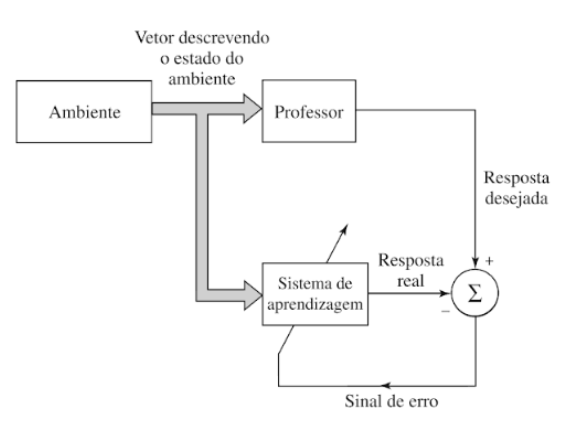
\includegraphics[scale=0.5]{AprendizadoSupervisionado}
 \end{center}
 \legend{Fonte: \citeauthor{haykin2009neural}, \citeyear{haykin2009neural}} 
 \end{figure}
 
 Nesta classe de algoritmos há uma diferente dissociação entre aqueles que lidam com rótulos discretos, cujos problemas são conhecidos como classificação, e aqueles que lidam com rótulos contínuos, cujos problemas são conhecidos como regressão. 
 
 Nos problemas de classificação, o objetivo é classificar as entradas em categorias. Por exemplo, um sistema que distingue o modelo de carros baseado em fotos. Para problemas de regressão, os resultados obtidos do sistema formam uma função contínua. Um exemplo seria um sistema que calcula o valor de uma moeda nos próximos 30 dias baseado na sua flutuação durante o mês anterior. Na Figura \ref{fig:classregres} é apresentado um exemplo conceitual da diferença entre classificação e regressão.
 
 \begin{figure}[htb]
 \caption{\label{fig:classregres} Distribuição de dados de classificação e regressão}
 \begin{center}
 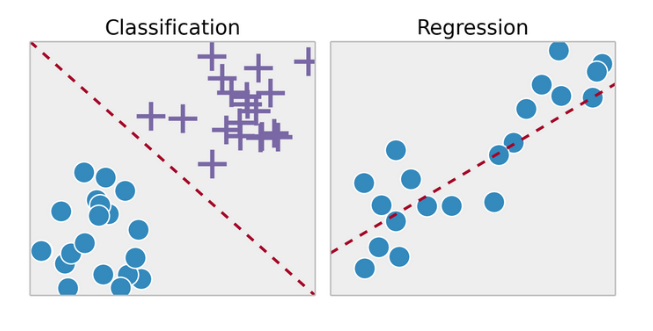
\includegraphics[scale=0.75]{ClassificacaoRegressao}
 \end{center}
 \legend{Fonte: \citeauthor{mediummachine}, \citeyear{mediummachine}} 
 \end{figure}


\section{Aprendizado Não Supervisionado}
\label{sec:nsuperv}

 No aprendizado não supervisionado o sistema é treinado com amostras não necessariamente rotulados e sem conhecimento da melhor saída possível \cite{haykin2009neural}. Por isso, a adaptação é feita a partir de uma medida independente da tarefa que mede a qualidade da representação do que o sistema deve aprender \cite{beckerneural}, por não ser possível realizar comparações com a resposta ideal para se determinar um erro. 

 Por exemplo no método de agrupamento, o sistema analisa as amostras fornecidas e as separa em grupos baseado em propriedades semelhantes encontradas. Este tipo de aprendizado é aplicável à problemas onde se deseja descobrir características relevantes nos dados de entrada \cite{goldschmidt}, porém os grupos não necessariamente apresentam informações relevantes, muitas vezes precisando de um estudo para verificar sua validade.\cite{Monard2003a} 

 Um exemplo de aplicação de técnicas de agrupamento é um sistema que analisa informações sobre vários pacientes de um hospital para tentar descobrir novos sintomas para uma determinada doença, que posteriormente são estudados por um médico para verificar se a doença em caso realmente têm relação com os sintomas encontrados.

 Na Figura \ref{fig:comparacaoaprendizado} é representado um exemplo da diferença entre o aprendizado supervisionado e não supervisionado, onde o supervisionado classifica cada saída com um rótulo e o não supervisionado agrupa as saídas de acordo com padrões. 


 \begin{figure}[htb]
 \caption{\label{fig:comparacaoaprendizado} Comparaçao entre aprendizados}
 \begin{center}
 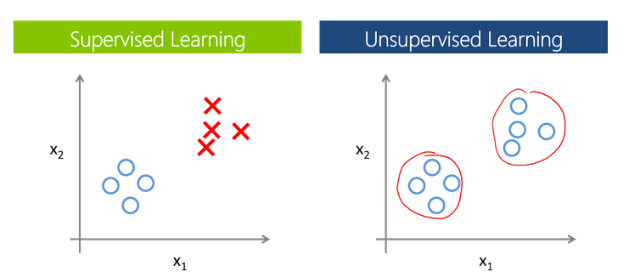
\includegraphics[scale=0.75]{ComparaAprendizado}
 \end{center}
 \legend{Fonte: \citeauthor{mediummachine}, \citeyear{mediummachine}} 
 \end{figure}

%\autoref{chap:cap1}
% ---
%\section{Aliquam vestibulum fringilla lorem}
%\lipsum[2]
%\subsection{Subsessão cap 1}
%\lipsum[2]
%\chapter{Capitulo Segundo}
%\lipsum[2]

\chapter{Desenvolvimento do Projeto}
\label{chap:desenv}

As ferramentas escolhidas para o desenvolvimento do projeto foram a Unity3D para a criação da aplicação, ASP.NET Core para a REST API e React para o dashboard administrativo.
 
\section{Estrutura}
\label{sec:estrutura}

A figura 3.1 demostra o fluxo de dados entre os componentes do projeto, os clientes (Web ou Unity) fazem requisições  para uma API que busca ou guarda os dados em um banco de dados relacional (SQL Server) e retorna o resultado da operação.

\begin{figure}[htb]
\caption{\label{fig:estrutura} Fluxo De Dados }
\begin{center}
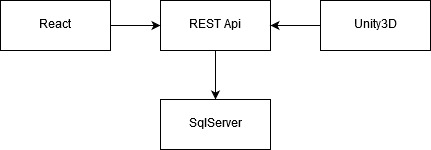
\includegraphics[scale=0.75]{estrutura}
\end{center}
\legend{Fonte: própria} 
\end{figure}


\section{REST API}
\label{sec:restapi}


A API serve como centro do projeto. Ela guarda todas as questões, usuários, opções e os rankings. Ela decide também quais e quantas questões um jogador irá receber quando uma nova partida for requisitada. 
Os clientes e a API se comunicam utilizando o protocolo Http\cite{fielding_reschke_2014} através do protocolo rest  REST\cite{wwrest}, enviando e recebendo JSONs.

A API é implementado em C\# utilizando o ASP NET Core 2.2\cite{aspnetcore} e Entity Framework Core\cite{entityFramework} para acesso ao banco de dados.

\subsection{Usuários}
\label{subsec:usuários}

Os usuários são representados pela classe user. Cada usuário tem um Username único e uma lista de roles que determinam quais funcionalidades da API o usuário tem acesso. A senha do usuário é passada pelo algoritmo HMAC-SHA521\cite{rcfHAMAC} e somente o hash resultante e o salt utilizados são salvos no banco.

Um usuário pode ser tanto um jogador como um administrador, podendo ser ambos dependendo das Roles dadas ao usuário. 

A função da API para criação de usuários é a aberta, por tanto qualquer um pode se registrar, porém usuários criados assim só terão acesso às funções de jogador. Um administrador pode depois dar a um usuário acesso às funções de administração.

\subsection{Controle de Acesso}
\label{subsec:acesso}

Cada função da API restringe seu acesso dependendo das Roles que ela requer de um usuário acessado. Existem 2 Roles no sistema “admin” e “user” que dão acesso às funções de administração e às funções do jogo respectivamente.

Algumas funções não requerem um usuário logado, como a função de cadastro e login, e outras só requerem que o usuário esteja logado, sem se importar com quais Roles eles possuem.

\subsection{Questões}
\label{subsec:questoes}

Cada questão possui um enunciado, uma flag indicando se essa questão está ativa e deveria ser enviada aos jogadores e um número aleatório utilizando para escolha das questões para um jogador. Opcionalmente uma questão pode ter uma imagem e varios Temas e Categorias. 

Cada questão deve ter exatamente 4 respostas com somente uma sendo marcada como correta para poder ser marcada como ativa. 

\subsubsection{Respostas}
\label{subsubsec:respostas}

Cada resposta tem um texto, uma flag indicando se essa resposta é correta e opcionalmente uma imagem. 

Uma resposta está sempre ligada a uma única questão e somente uma resposta ligada a cada questão pode ser marcada como correta. 


\subsubsection{Escolhendo Questões}
\label{subsubsec:escolhendo}

Quando um jogador começa uma nova partida a API escolhe quais questões para enviar para o jogador. A escolha é feita aleatoriamente entre as questões ativas que o jogador ainda não tenha respondido. 

Primeiramente as questões são filtradas para conterem somente questões ativas que o jogador não tenha respondido ainda. Depois um número aleatório é gerado e é feito um “ou exclusivo” entre este número e o número aleatório de cada questão e as questões são ordenadas de acordo com os números resultantes. Por fim a quantidade necessária de questões é pega a partir do começo da lista.

Caso depois do processo não existam questões suficientes para uma partida, a lista de questões que o jogador já respondeu é apagada e o processo é repetido excluindo as questões que já tenham sido escolhidas anteriormente e o número de questões faltando são escolhidas. Se mesmo assim não houverem questões suficientes a partida começa com questões faltando.

\subsection{Partidas}
\label{subsec:partidas}

Uma partida começa com o jogador requisitando o começo de uma nova partida para a API e recebendo as questões a serem respondidas. 

Uma vez que o jogador tenha respondido a todas as questões ele manda as respostas escolhidas de volta para a API que calcula quantos pontos o jogador fez nesta partida e quais questões foram respondidas.

Os pontos são adicionados a cada ranking e o total de pontos conseguidos e a nova classificação nos rankings é retornado ao jogador.

\subsection{Rankings}
\label{subsec:rankings}

O jogo possui 3 rankings por padrão, um semanal, um mensal que são reiniciados a cada 7 dias e a cada 30 dias respectivamente e um perpétuo que nunca é reiniciado.     Administradores podem criar rankings adicionais com configurações diferentes. Os rankings são públicos e atualizados cada vez que uma partida termina.

\subsubsection{Reiniciando Rankings}
\label{subsubsec:reiniciando}

Os resultados dos rankings reiniciados não são perdidos. Ao invés de deletar os dados de um ranking, um novo ranking com o mesmo nome e duração é criado e o antigo é desativado, fazendo com que para os usuários o ranking seja reiniciado, mas para os administradores os dados ainda são acessíveis.

O processo de reiniciar os rankings é feito por um serviço periódico que roda a cada 30 minutos, porém um administrador pode reiniciar um ranking manualmente se desejado.

\section{Unity3D}
\label{sec:unity3d}

O desenvolvimento da aplicação do projeto foi feita utilizando a Engine de jogos Unity3D. As principais vantagens obtidas por escolher a Unity3D como ambiente de desenvolvimento foram: a facilidade de criar projetos
para plataformas diferentes utilizando a mesma base de código e design visual, um sistema intuitivo e visual de criação de telas e a familiaridade do Laboratória de Inovação de Games e Apps.(LIGA) com projetos feitos com a engine para suporte posterior.

\subsection{Telas}
\label{subsec:telas}

O design da aplicação foi montada para utilizar apenas uma cena dentro da Unity3D, isso faz com que não tenha tempo perdido para carregar outras telas durante a execução da aplicação, deixando-a mais responsiva para o usuário.

Não foram utilizados muitos elementos nas telas da aplicação para que o cliente possa customizar de acordo com o visual de seu negócio, modificando a paleta de cores e a disposição de logomarcas dentro da aplicação.

No total a aplicação conta com sete telas completas e dois elementos de suporte.

\subsubsection{Base}
\label{subsubsec:base}

A tela base consiste em uma cor padrão que preenche todo a parte de fundo da aplicação que pode ser modificada pelo cliente ou substituída por uma logomarca, e uma barra localizada na parte superior que contém o nome do usuário ativo, sua pontuação geral e o horário atual.

Todas as telas seguintes ficarão localizadas à frente da tela de fundo e sempre embaixo da barra superior, sendo essa sempre visível ao usuário.

\subsubsection{Login}
\label{subsubsec:login}

A tela de login é a tela principal, enquanto não há interação com a aplicação e após um usuário finalizar sua sessão ela ficará exposta. A tela contém três elementos.
    
O elemento central consiste em dois campos para serem preenchidos, um com o usuário e o outro com senha, e um botão para realizar o processo de login. Quando o usuário interagir com esse botão, caso algum dos campos esteja vazio, uma mensagem de erro aparecerá com uma mensagem informando o usuário para ele preencher todos os campos. Caso todos os campos estejam preenchidos, uma chamada para a API é feita, caso os valores estejam corretos o usuário é direcionado para a tela de seleção de temas para começar a experiência. Se as informações de login não estejam certas, uma mensagem de erro informando que os valores estão errados será mostrado ao usuário.

Os outros dois elementos consistem e dois botões localizados nos cantos da tela.
    
O botão no canto direito superior leva o usuário para a tela de ranking, onde ele poderá verificar a colocação de todos os usuários sem a necessidade de fazer login com uma conta.
    
O botão no canto direito inferior leva o usuário para a tela de cadastro.

\subsubsection{Cadastro}
\label{subsubsec:cadastro}

A tela de cadastro contém uma área com campos necessários para a criação de uma nova conta, um botão para criar a conta com as informações informadas e um botão para retornar para a tela de login.


\subsubsection{Lobby}
\label{subsubsec:lobby}

Após o usuário realizar o login ele será redirecionado para a tela de lobby onde ele poderá iniciar uma sessão de perguntas para verificar seu conhecimento em uma área de trabalho. O usuário também tem acesso ao ranking e a possibilidade de voltar à tela de login, removendo o vínculo de sua conta com a sessão atual.


\subsubsection{Ranking}
\label{subsubsec:rankingunity}

A tela de ranking contém uma lista mostrando os melhores colocados em cada ranking.


\subsubsection{Perguntas}
\label{subsubsec:perguntasunity}

A tela de perguntas é separada em duas partes, a área que mostra a pergunta escolhida pelo sistema, e a área dedicada às respostas que o usuário pode escolher.

A parte separada para a pergunta possui espaço suficiente para conter uma imagem e um pequeno texto explicativo para melhor entendimento do usuário. Esta parte é adaptativa e pode mudar seu tamanho dependendo do tamanho e quantidade de elementos presentes.

As respostas podem estar dispostas de duas maneiras. A primeira é como uma lista vertical caso as respostas sejam compostas somente por texto, deixando um espaço maior no eixo horizontal para deixa a leitura mais simples. Na segunda disposição, cada resposta ocupa um canto da área. Essa disposição permite que as respostas tenham uma imagem e um espaço para uma pequena descrição.

O usuário precisa escolher uma resposta, que ficará marcada como selecionada, e em seguida, precisa interagir com o botão “Próximo” para enviar sua seleção para o servidor. Logo em seguida, a resposta correta será indicada para o usuário, tendo um feedback instantâneo sobre sua escolha.

Quando o usuário estiver na última pergunta de uma partida o botão “Próximo” muda para mostrar o texto “Terminar” e quando o usuário receber o feedback da resposta escolhida, ele será redirecionado para a tela de resultados.


\subsubsection{Resultado}
\label{subsubsec:resultado}

A tela de resultados mostra a performance do usuário após responder as perguntas de uma sessão, informando-o do resultado da resposta de cada pergunta, o número de acertos em relação ao total de perguntas e a pontuação geral obtida na sessão.


\subsubsection{Carregando}
\label{subsubsec:carregando}

A tela de carregando aparece toda vez que alguma operação que requer que usuário espere uma resposta. Esta tela aparece na frente de todas as outras e impede que o usuário interaja com a aplicação até receber uma resposta.


\subsubsection{Erros}
\label{subsubsec:erros}

A janela de erros aparece na frente de todas as outras telas informando o usuário que algo de errado aconteceu junto de um botão que fecha a janela.

\subsection{Scriptable Objects Architecture}
\label{subsec:scriptableobjectsarch}

No desenvolvimento da aplicação foram aplicados os conceitos sobre a utilização de Scriptable Object como base da arquitetura geral. O conceito
As transições e comunicação entre scripts são feitas por meio de eventos que persistem durante a execução da aplicação como Scriptable Objects.

\subsubsection{Scriptable Objects}
\label{subsubsec:scriptableobjects}

Um ScriptableObject é um contêiner de dados utilizado para salvar grandes quantias de dados, independente de instâncias de classes. Um dos principais casos de uso para ScriptableObjects é para reduzir a utilização de memória de um projeto por evitar a cópia de valores entre múltiplos objetos.\cite{scriptableobject}


\subsubsection{Game Events}
\label{subsubsec:gameevents}

Lorem Ipsum


\subsection{Acesso à API}
\label{subsec:acessoapi}

O acesso a API é feito através da biblioteca LigaFit. A LigaFit, inspirado pelo RetroFit mas implementado para Unity3D e levando em conta as características das plataformas normalmente utilizadas pelo LIGA, permite que a API seja descrita através de uma interface e gera implementação automaticamente.


\section{React}
\label{sec:react}
As funções administrativas são disponibilizadas para o usuário através de um web site desenvolvido em React\cite{react}. O web site permite a um usuário administrador gerir as questões e usuários e obter informações sobre a taxa de acertos e erros das questões. 

\subsection{Login}
\label{subsec:loginreact}

A tela de login possui campos para o Username e a senha do usuário, além de uma opção para lembrar do login em visitas futuras.

Qualquer usuário pode logar no web site, porém somente os que tenham credenciais de administrador terão acesso a maioria das funções.


\subsection{Questões}
\label{subsec:questoesreact}

O web site  mostra a lista de questões em ordem alfabética, junto com se a questão está ativa.
    
O usuário pode selecionar uma questão e ser redirecionado a tela de detalhes da questão.


\subsubsection{Detalhe da Questão}
\label{subsubsec:detalhequestao}

A tela de detalhes de questão permite que o usuário edite o enunciado da questão, se ela está ativa, a imagem da questão e mostra e permite a edição das respostas da questão.


\subsubsection{Relatório das Questões}
\label{subsubsec:relatorioquestoes}

Nesta tela o administrador pode ver um relatório sobre todas as questões, que mostra quantas vezes cada questão foi respondida e quantos erros, acertos e pulos uma questão teve. O relatório é pode ser configurado para mostrar informações de  qualquer período de tempo que o administrador deseje.

\subsection{Configurações}
\label{subsec:configreact}

Esta tela permite que o administrador ajuste as configurações do jogo, podendo decidir quantas questões uma partida deve ter, quantos pontos cada questão vale em novas partidas.

\subsection{Rankings}
\label{subsec:rankingsreact}

O ranking semanal, mensal e perpétuo são mostrados nesta tela. Como os rankings são públicos, essa tela não requerer que o usuário esteja logado para ser acessada.

\subsection{Usuários}
\label{subsec:usuariosreact}

Os administradores podem visualizar todos os usuários da plataforma, podendo criar, editar e deletar usuários.
\chapter{Resultados}
\label{chap:resultados}

Apresenta a plataforma gamificada, explicando as funcionalidades e como elas são úteis para o aprendizado em uma empresa.
 


% ----------------------------------------------------------
% Finaliza a parte no bookmark do PDF
% para que se inicie o bookmark na raiz
% e adiciona espaço de parte no Sumário
% ----------------------------------------------------------
\phantompart

% ---
% Conclusão
% ---
\chapter{Conclusão}
\label{chap:conclusao}


% ----------------------------------------------------------
% ELEMENTOS PÓS-TEXTUAIS
% ----------------------------------------------------------
\postextual
% ----------------------------------------------------------

% ----------------------------------------------------------
% Referências bibliográficas
% ----------------------------------------------------------
\bibliography{pos-textuais/bibliografia}

% ----------------------------------------------------------
% Glossário
% ----------------------------------------------------------
%
% Consulte o manual da classe abntex2 para orientações sobre o glossário.
%
%\glossary

% ----------------------------------------------------------
% Apêndices
% ----------------------------------------------------------

% ---
% Inicia os apêndices
% ---

% ---
\begin{apendicesenv}

% Imprime uma página indicando o início dos apêndices
%\partapendices

% ----------------------------------------------------------
\lstset{frame=none}
\chapter{\textit{Alpha GO}}
\label{ap:alphago}



\end{apendicesenv}

% ----------------------------------------------------------
% Anexos
% ----------------------------------------------------------

% ---
% Inicia os anexos
% ---
%\begin{anexosenv}

% Imprime uma página indicando o início dos anexos
%\partanexos

% ---
%\chapter{Morbi ultrices rutrum lorem.}
% ---
%\lipsum[30]

% ---
%\chapter{Cras non urna sed feugiat cum sociis natoque penatibus et magnis dis
%parturient montes nascetur ridiculus mus}
% ---

%\lipsum[31]

% ---
%\chapter{Fusce facilisis lacinia dui}
% ---

%\lipsum[32]

%\end{anexosenv}

%---------------------------------------------------------------------
% INDICE REMISSIVO
%---------------------------------------------------------------------
%\phantompart
\printindex
%---------------------------------------------------------------------

\end{document}
